% \begin{figure*}[t]
%     \centering
%     \includegraphics[width=0.95\linewidth]{image/img/kgqa_for_kgc.pdf}
%     \caption{Ablation study of the effect of KBQA components
% in JQCL}
%     \label{Effect Analysis of Interaction For KGQA}
% \end{figure*}

% \begin{figure*}[t!]
%     \centering
%     \subfigure[]{
%         \label{subfig:(a)}
%         \includegraphics[width=0.235\textwidth]{image/img/kgqa_for_kgc/kgqa_for_kgc_11.pdf}}
%     \subfigure[]{
%        \label{subfig:(b)}
%         \includegraphics[width=0.235\textwidth]{image/img/kgqa_for_kgc/kgqa_for_kgc_12.pdf}}
%     \subfigure[]{
%        \label{subfig:(c)}
%         \includegraphics[width=0.235\textwidth]{image/img/kgqa_for_kgc/kgqa_for_kgc_13.pdf}}
%     \subfigure[]{
%        \label{subfig:(d)}
%         \includegraphics[width=0.235\textwidth]{image/img/kgqa_for_kgc/kgqa_for_kgc_14.pdf}}
%     \subfigure[]{
%        \label{subfig:(e)}
%         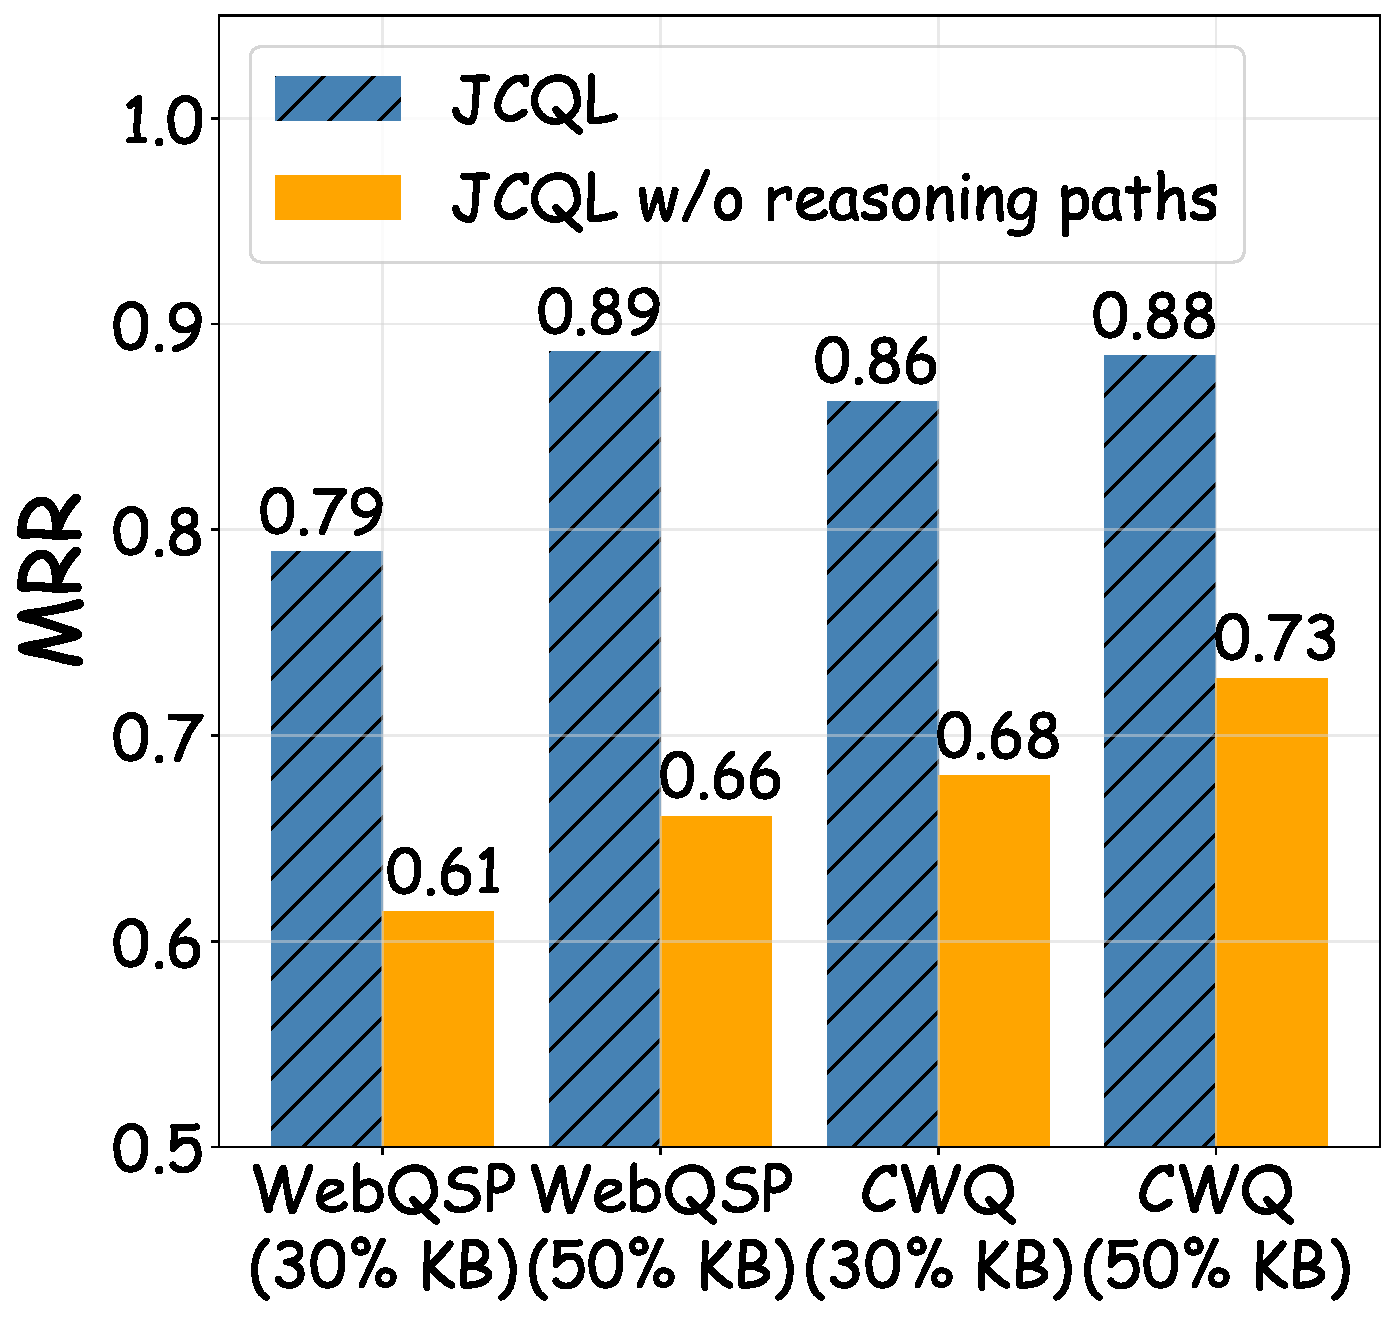
\includegraphics[width=0.235\textwidth]{image/img/kgqa_for_kgc/kgqa_for_kgc_21.pdf}}
%     \subfigure[]{
%        \label{subfig:(f)}
%         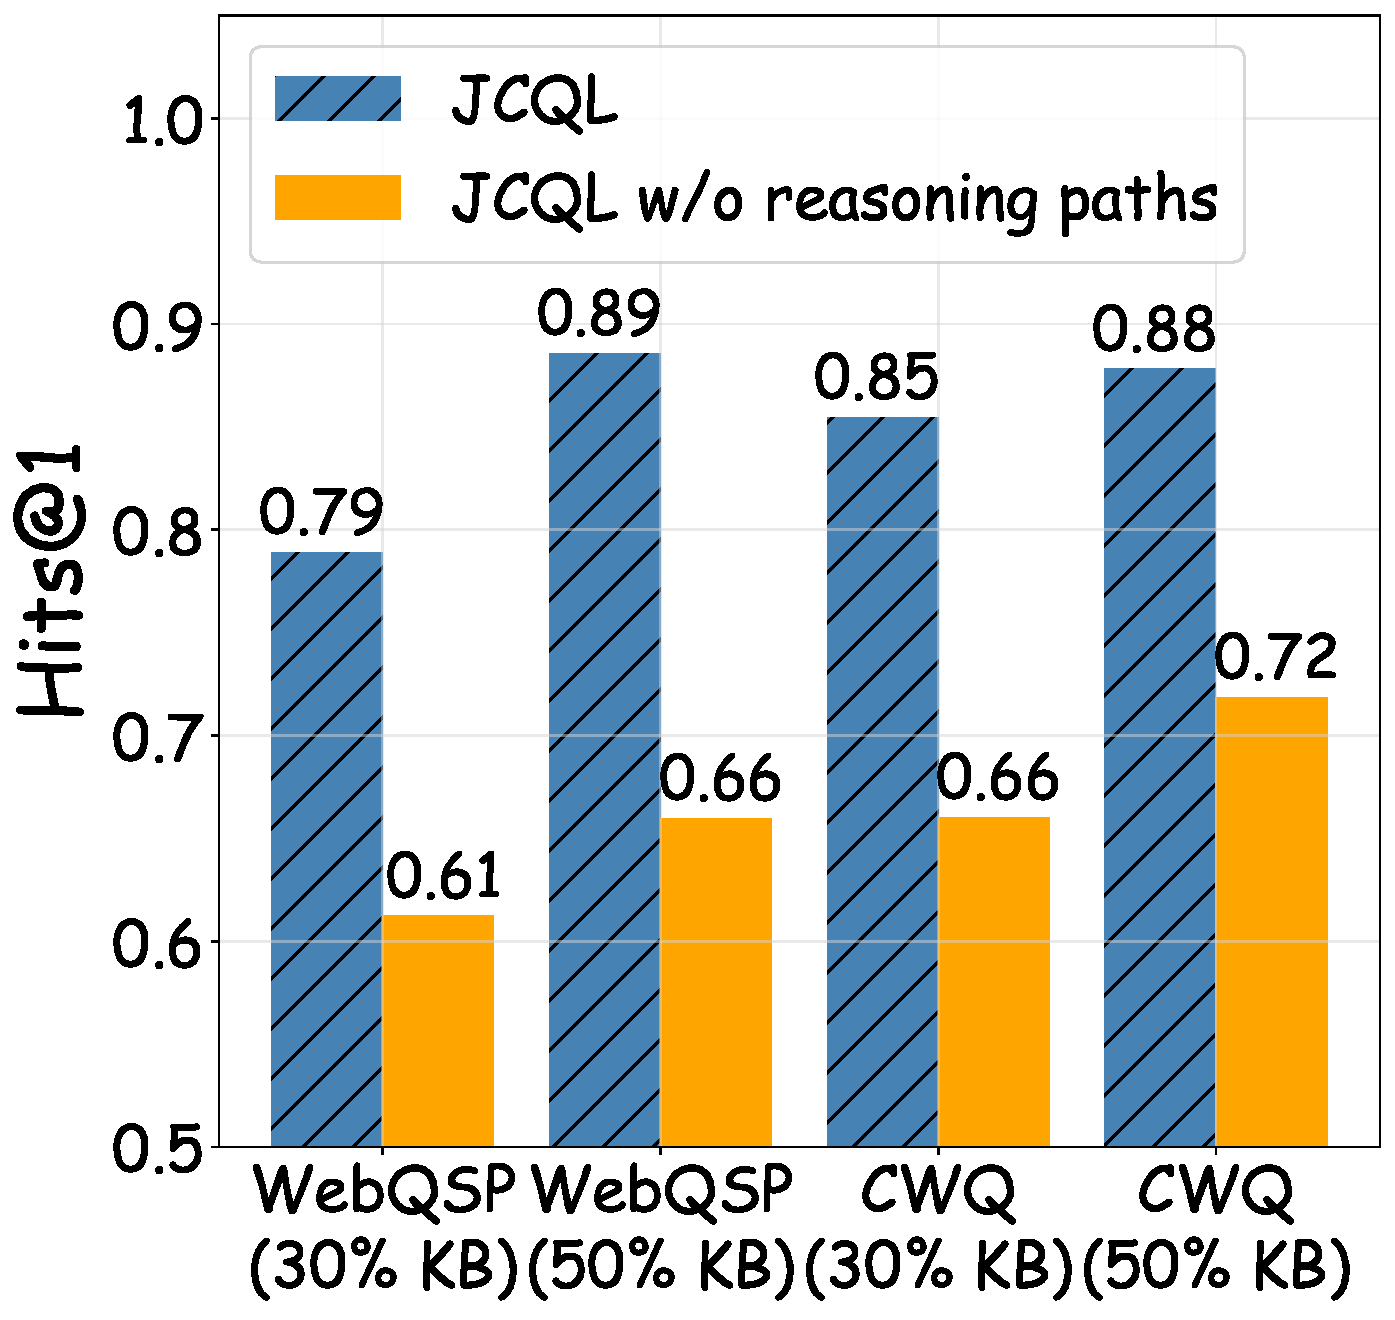
\includegraphics[width=0.235\textwidth]{image/img/kgqa_for_kgc/kgqa_for_kgc_22.pdf}}
%     \subfigure[]{
%        \label{subfig:(g)}
%         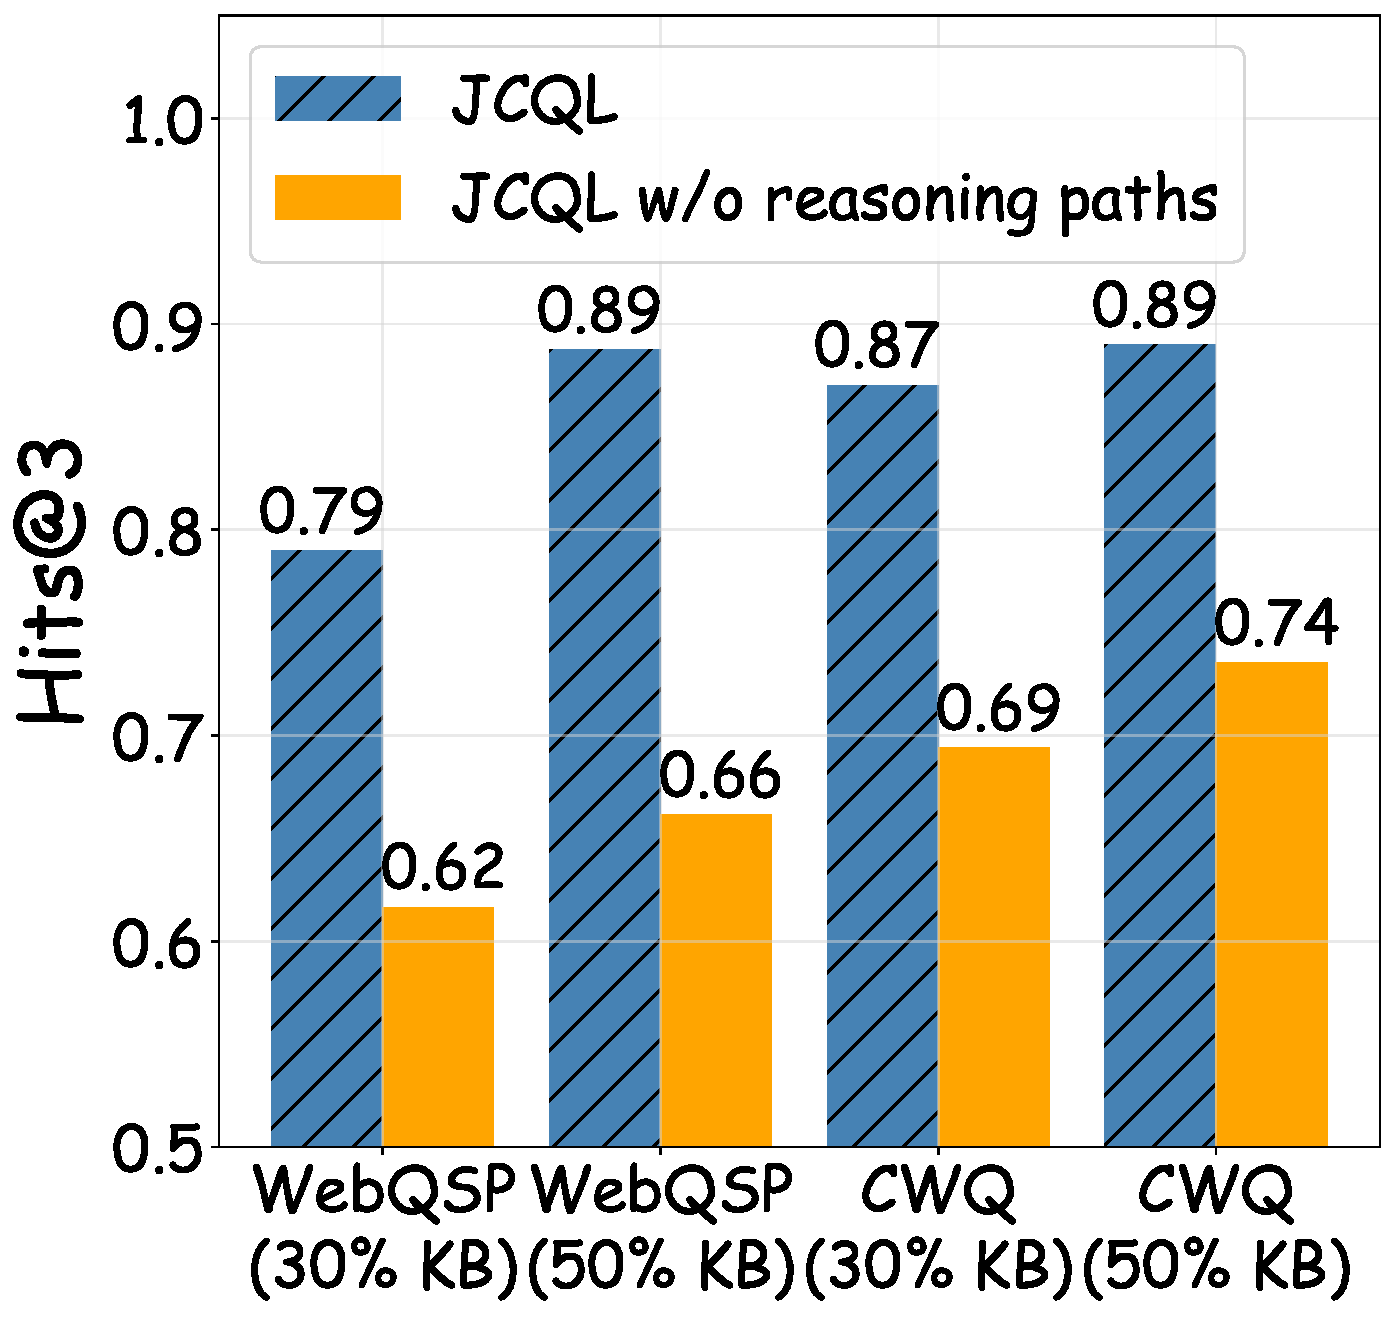
\includegraphics[width=0.235\textwidth]{image/img/kgqa_for_kgc/kgqa_for_kgc_23.pdf}}
%     \subfigure[]{
%        \label{subfig:(h)}
%         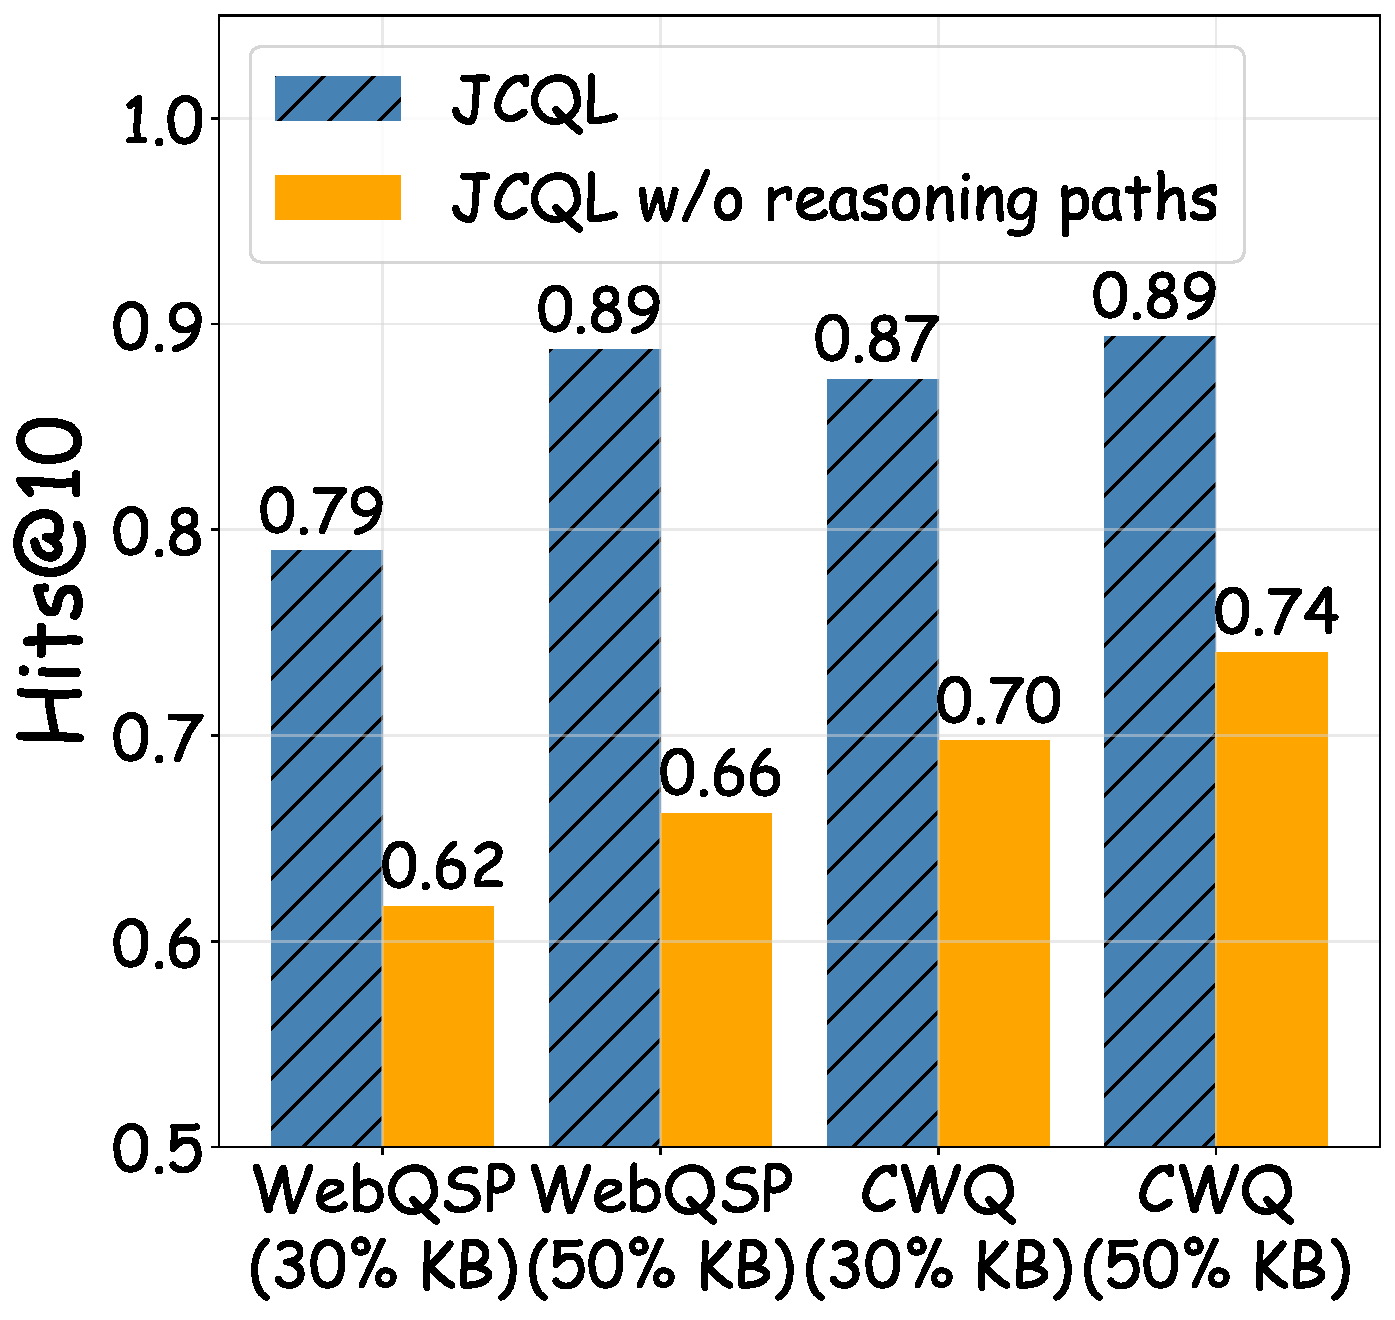
\includegraphics[width=0.235\textwidth]{image/img/kgqa_for_kgc/kgqa_for_kgc_24.pdf}}
%     \caption{Ablation study of the effect of the reasoning paths in JCQL.}
%     \vspace{-12pt}
%     \label{Effect Analysis of Interaction For KGC}
% \end{figure*}






\begin{figure*}[t!]
    \centering
    \subfigure[]{
       \label{subfig:(a)}
        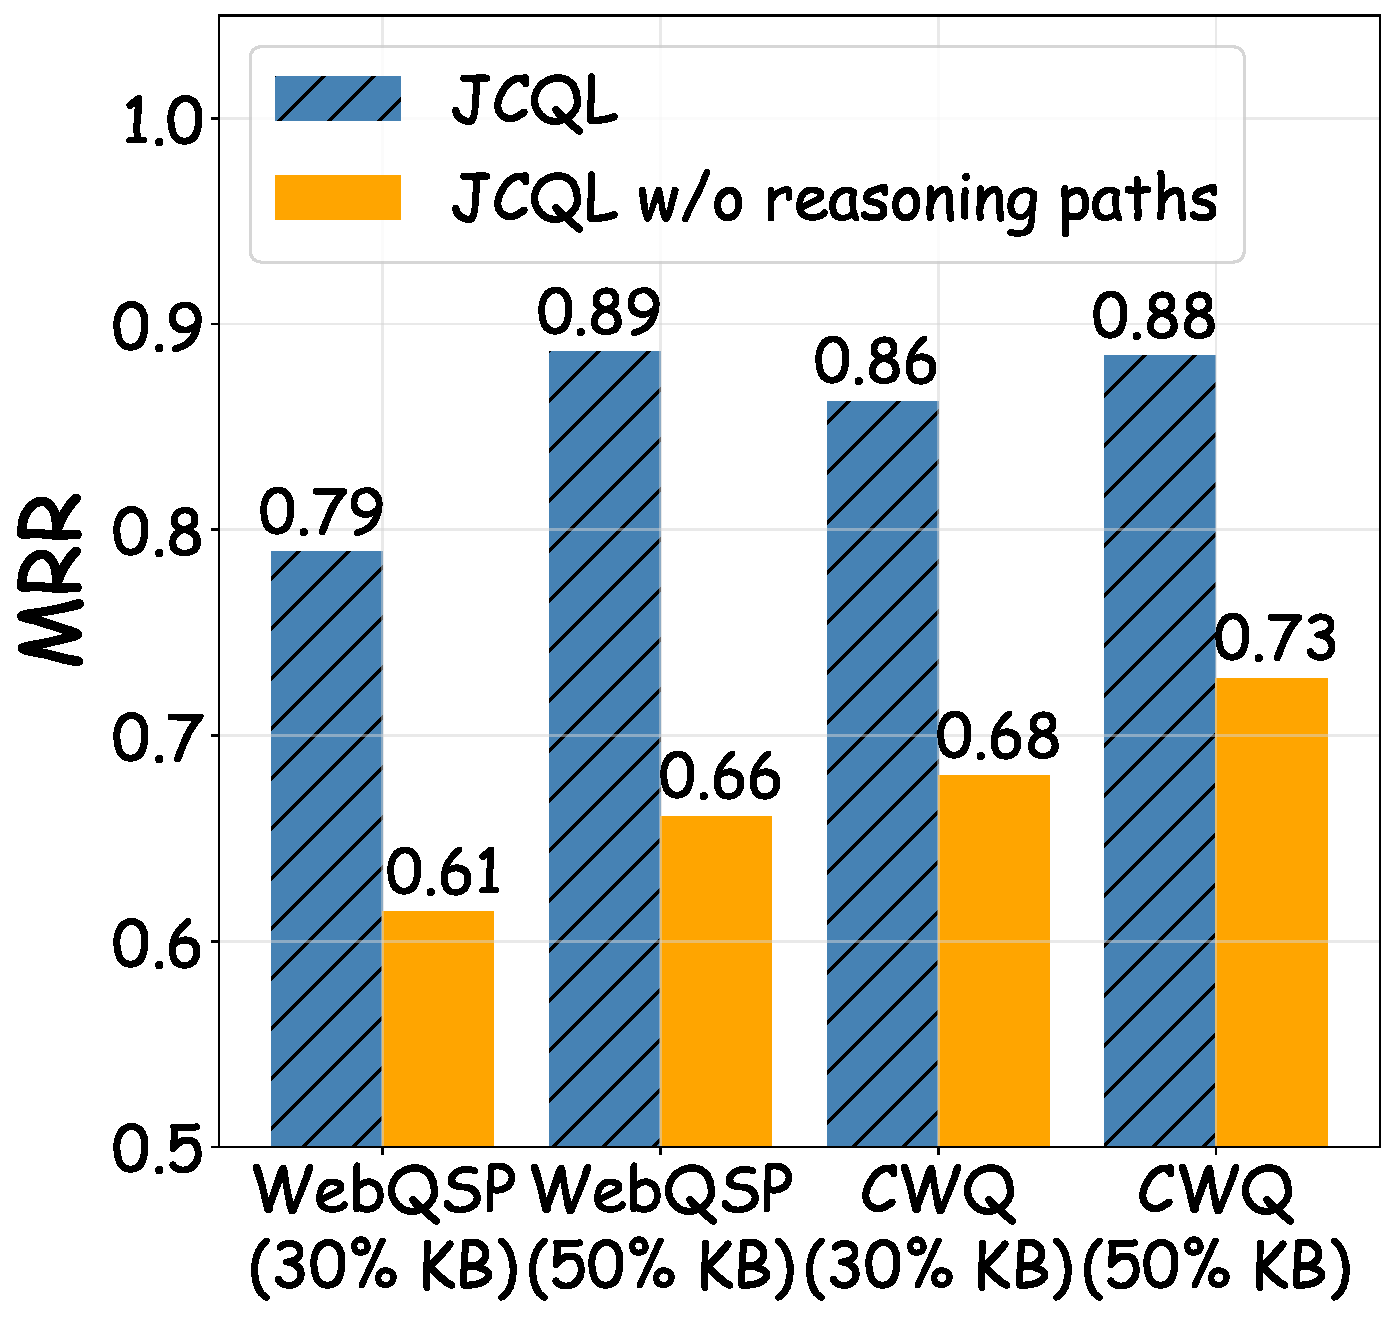
\includegraphics[width=0.22\textwidth]{image/img/kgqa_for_kgc/kgqa_for_kgc_21.pdf}}
    \subfigure[]{
       \label{subfig:(b)}
        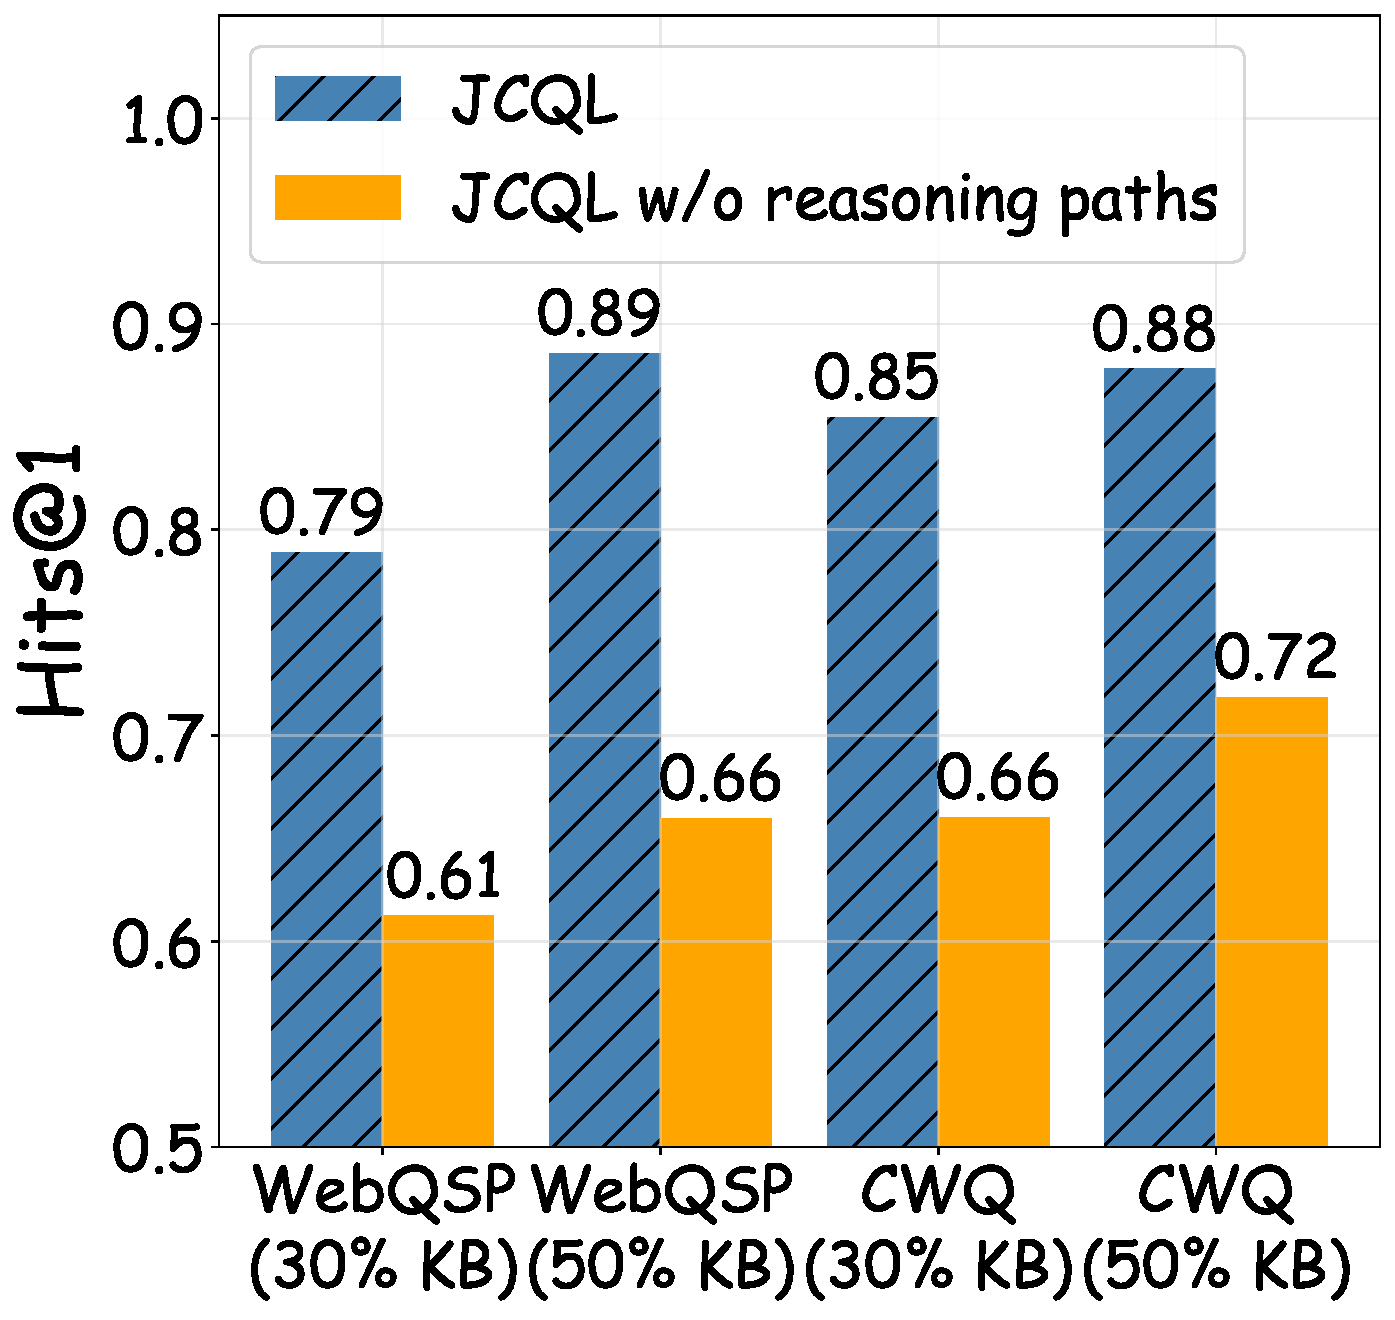
\includegraphics[width=0.22\textwidth]{image/img/kgqa_for_kgc/kgqa_for_kgc_22.pdf}}
    \subfigure[]{
       \label{subfig:(c)}
        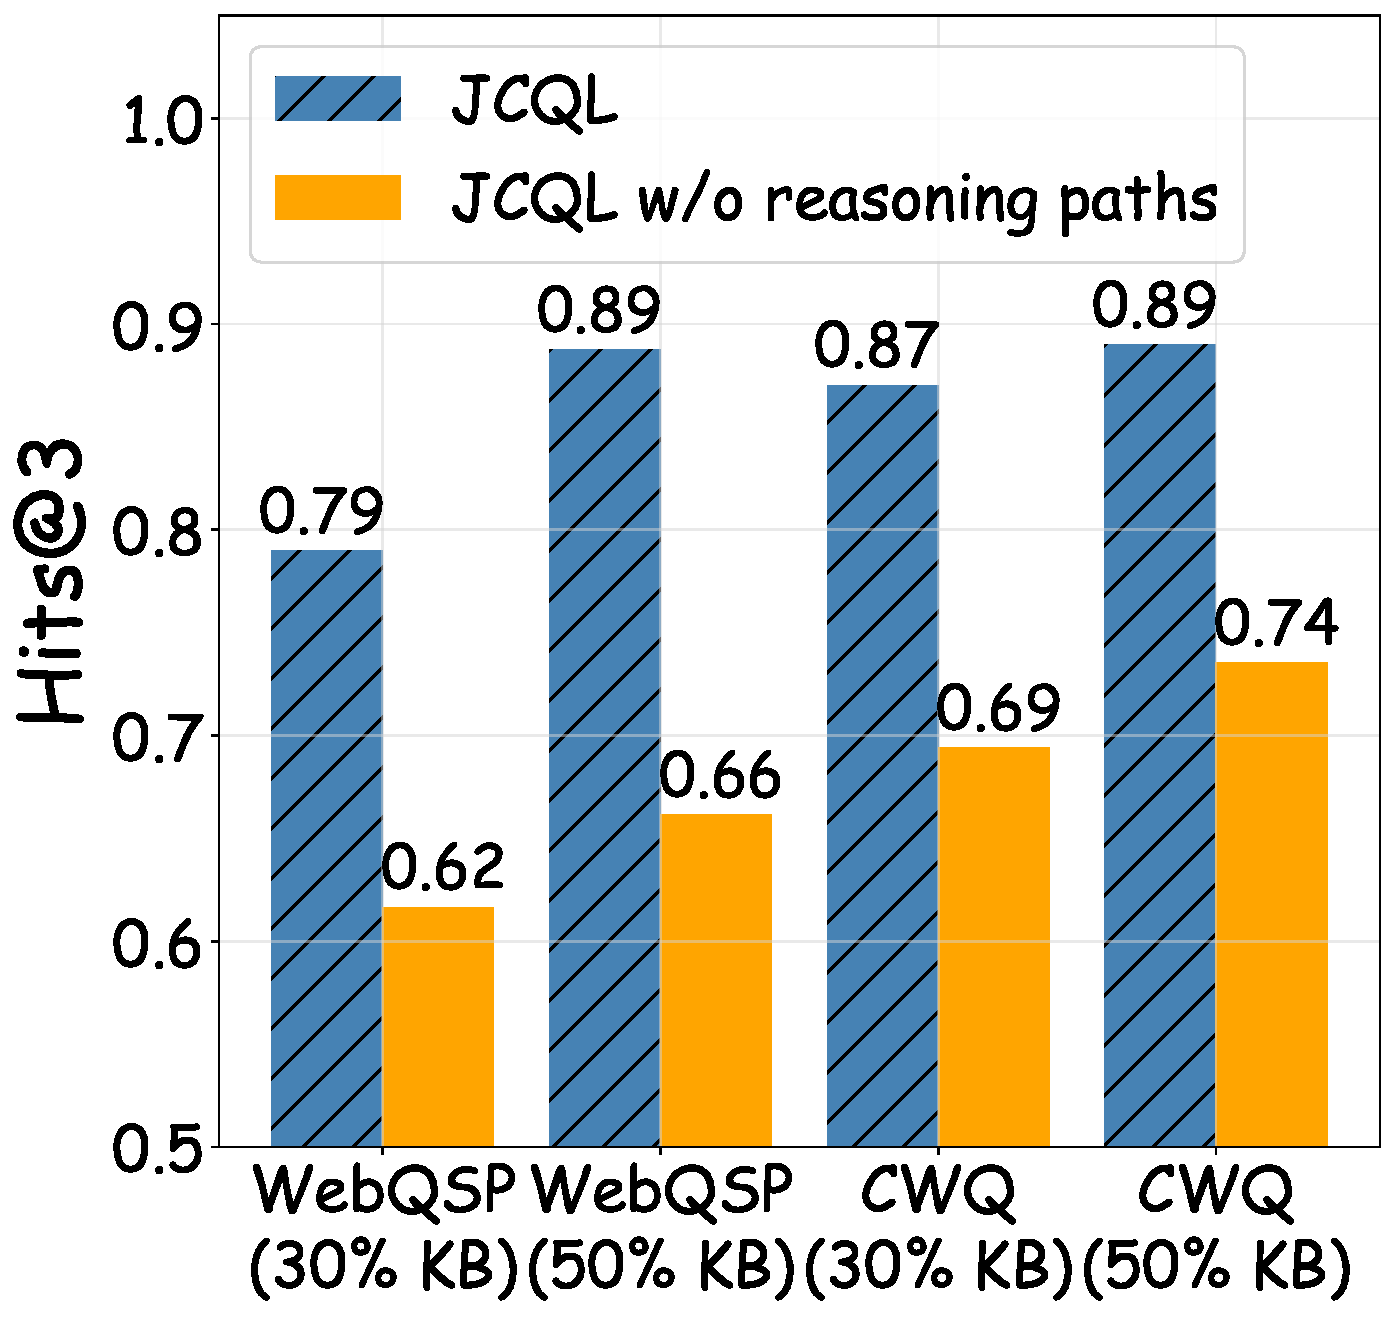
\includegraphics[width=0.22\textwidth]{image/img/kgqa_for_kgc/kgqa_for_kgc_23.pdf}}
    \subfigure[]{
       \label{subfig:(d)}
        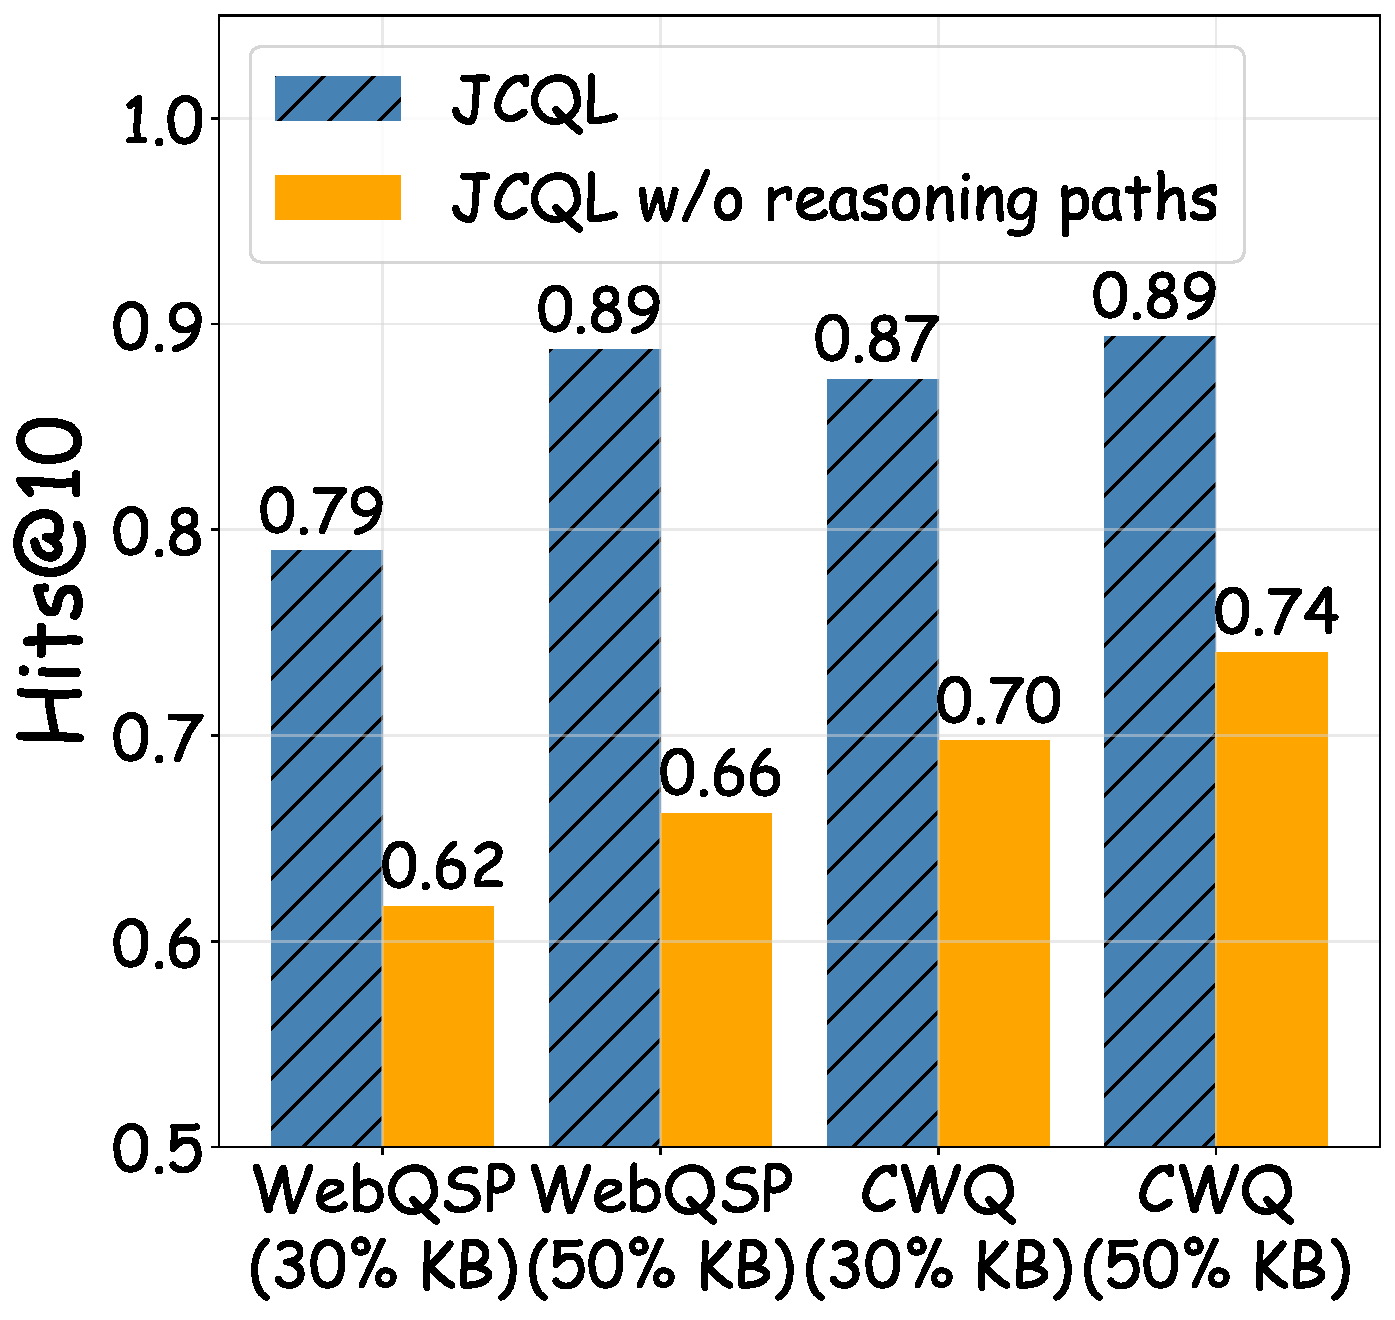
\includegraphics[width=0.22\textwidth]{image/img/kgqa_for_kgc/kgqa_for_kgc_24.pdf}}
    \caption{Ablation study on the LLM's reasoning paths for the task of KBC.}
    % \vspace{-5pt}
    \label{Effect Analysis of Interaction For KGC}
\end{figure*}


% 去掉hits10

% \begin{figure*}[t!]
%     \centering
%     \subfigure[]{
%        \label{subfig:(a)}
%         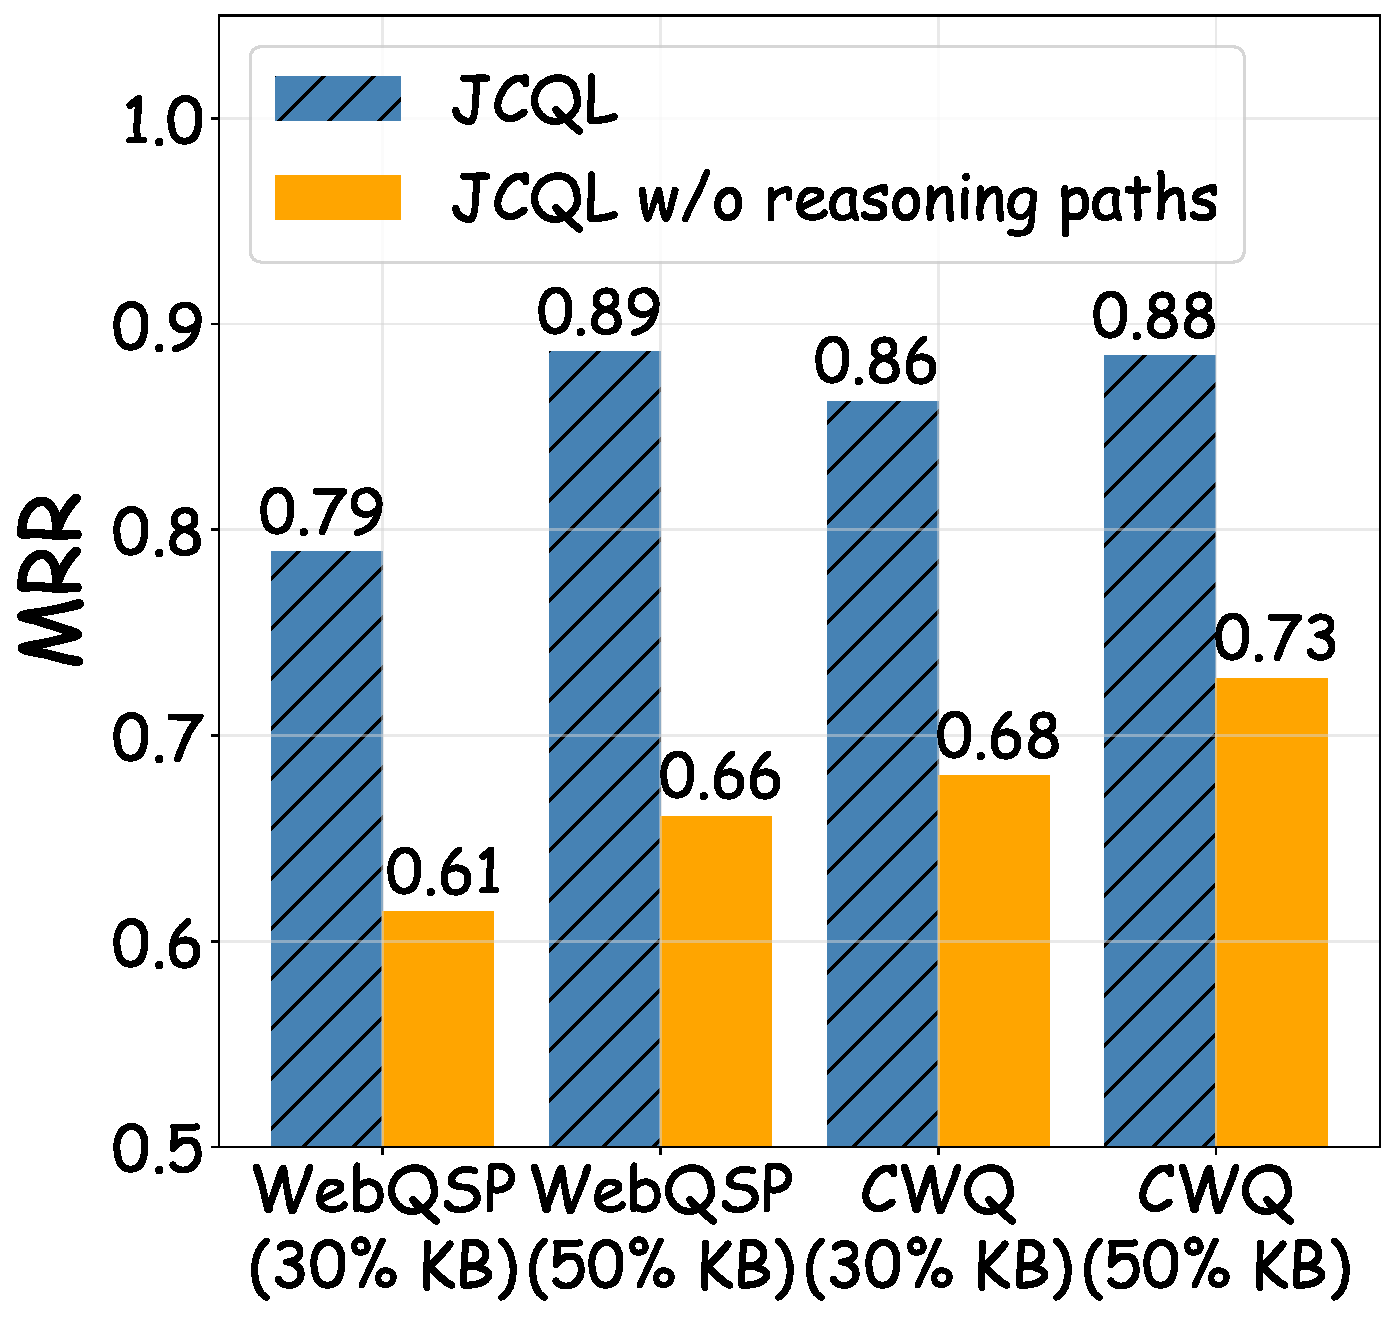
\includegraphics[width=0.24\textwidth]{image/img/kgqa_for_kgc/kgqa_for_kgc_21.pdf}}
%     \hspace{0.04\textwidth}
%     \subfigure[]{
%        \label{subfig:(b)}
%         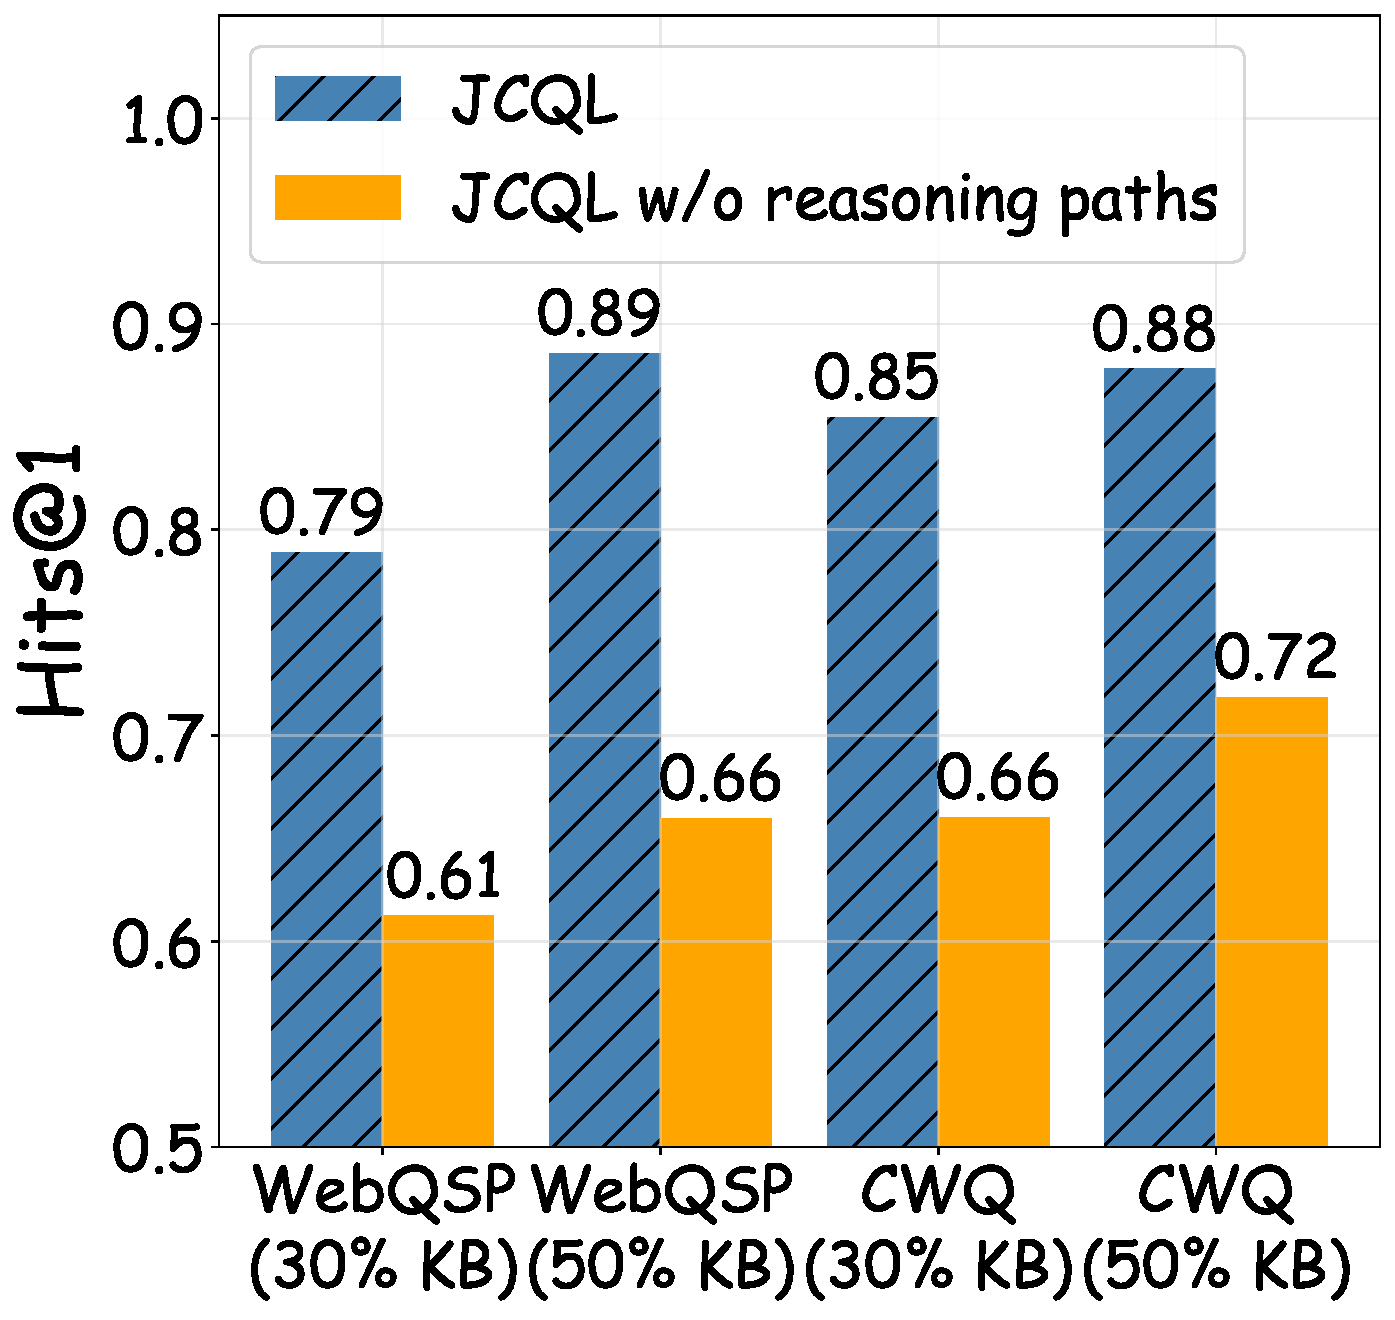
\includegraphics[width=0.24\textwidth]{image/img/kgqa_for_kgc/kgqa_for_kgc_22.pdf}}
%     \hspace{0.04\textwidth}
%     \subfigure[]{
%        \label{subfig:(c)}
%         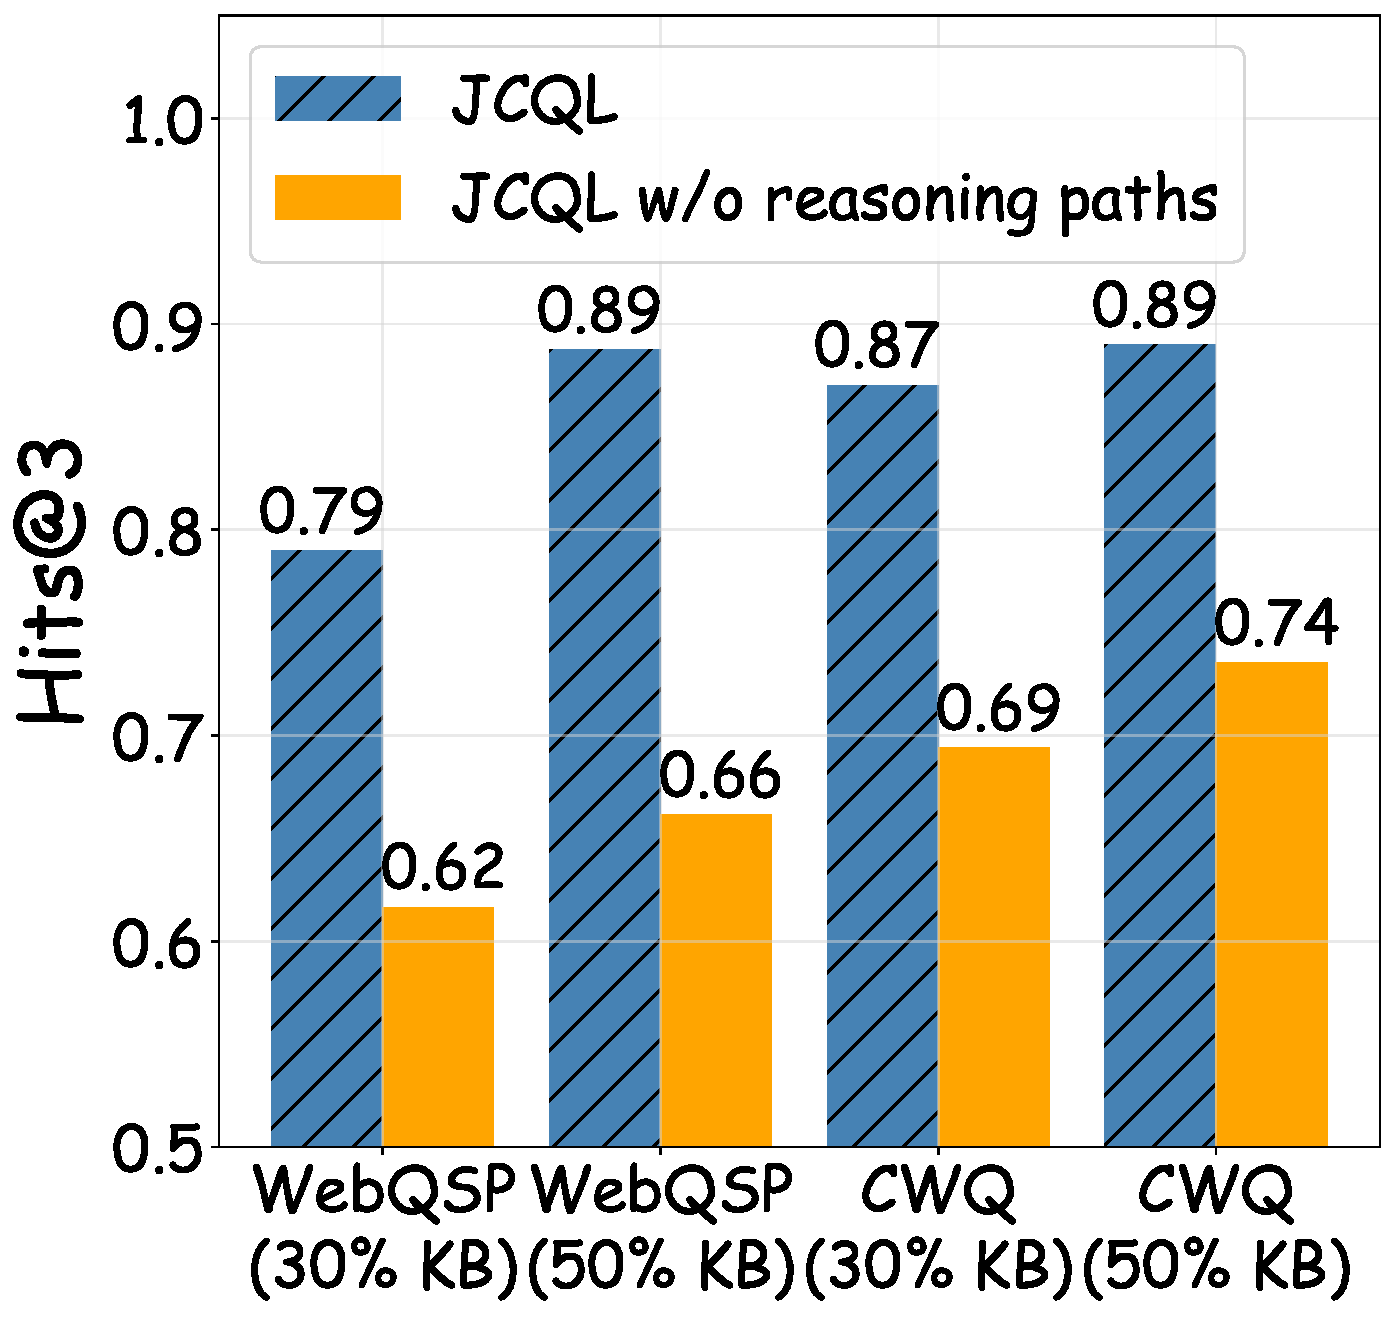
\includegraphics[width=0.24\textwidth]{image/img/kgqa_for_kgc/kgqa_for_kgc_23.pdf}}
%     % \vspace{-4pt}
%     \caption{Ablation study on the LLM's reasoning paths for the task of KBC.}
%     % \vspace{-4pt}
%     \label{Effect Analysis of Interaction For KGC}
% \end{figure*}